\documentclass[12pt,a4paper]{extarticle}
\usepackage[utf8]{inputenc}
\usepackage[T1]{fontenc}
\usepackage[dutch,shorthands=off]{babel}
\usepackage[margin=8mm]{geometry}
\usepackage{multicol}
\usepackage{listings}
\usepackage{xcolor}
\usepackage{enumitem}
\usepackage{titlesec}
\usepackage{lmodern}
\usepackage{array}
\usepackage{booktabs}
\usepackage{tikz}
\usetikzlibrary{decorations.pathreplacing, arrows.meta}

\setlength{\columnsep}{5mm}
\setlength{\parindent}{0pt}
\setlength{\parskip}{3pt}
\linespread{1.0}\selectfont
\setlist{nosep,leftmargin=4mm}

\definecolor{kw}{RGB}{0,0,160}
\definecolor{cm}{RGB}{100,100,100}
\definecolor{st}{RGB}{160,0,0}
\definecolor{hdr}{RGB}{20,60,120}

\titleformat{\section}{\bfseries\large\color{hdr}}{}{0pt}{}
\titlespacing{\section}{0pt}{8pt}{3pt}
\titleformat{\subsection}{\bfseries\normalsize}{}{0pt}{}
\titlespacing{\subsection}{0pt}{7pt}{2pt}

\lstset{
  language=Java,
  basicstyle=\ttfamily\small,
  keywordstyle=\color{kw}\bfseries,
  commentstyle=\color{cm}\itshape,
  stringstyle=\color{st},
  showstringspaces=false,
  columns=fullflexible,
  keepspaces=true,
  breaklines=true,
  breakatwhitespace=false,
  aboveskip=5pt,
  belowskip=6pt,
  xleftmargin=0mm
}

\pagestyle{empty}

\begin{document}

\begin{center}
    {\Large\bfseries Formularium Objectgerichte Softwareontwikkeling}\\[0.5mm]
    {\small Het examen is een race tegen de klok. Hier staat wat je het vaakst nodig
    hebt, om snel te vinden en verder te werken. Op het examen krijg je nog de java-docs.
    \texttt{docs.zip}.

    Source code vind je op \texttt{https://github.com/KUL-Industriele-ingenieurs/Samenvattingen-Ku-leuven-Industriele-ingenieurs}. Wees niet bang om
    dingen toe te voegen of te veranderen.}

    Vergeet niet om ctrl+space te gebruiken in Bluej voor autocomplete!
\end{center}
\vspace{1mm}

\begin{multicols}{2}

    %--------------------------------------------------------
    \section{1. Skelet van een klasse}
    \begin{lstlisting}
import java.util.ArrayList;

public class Quiz
{
    private String naam;
    private ArrayList<Ant> ants;

    // constructor: geen returntype
    public Quiz(String naam)
    {
        this.naam = naam;
        // lijst hier aanmaken!
        ants = new ArrayList<>();
    }

    public String getNaam()
    {
        return naam;
    }
    public void setNaam(String n)
    {
        naam = n;
    }
}
// velden private, methodes public
// hulpmethode voor jezelf: private
\end{lstlisting}
    De lijst moet je in de constructor aanmaken, anders krijg je een
    \emph{NullPointerException}. In de punthaken staat een klasse, dus
    \texttt{<Integer>} en nooit \texttt{<int>}.

    \textbf{Constante:}
    \begin{lstlisting}
public static final int MAX = 10;
\end{lstlisting}

    %--------------------------------------------------------
    \section{2. Types}
    \begin{center}
        \small
        \begin{tabular}{@{}ll@{}}
            \toprule
            \texttt{int}     & \texttt{5}                     \\
            \texttt{double}  & \texttt{5.0}                   \\
            \texttt{float}   & \texttt{5.0f}                  \\
            \texttt{boolean} & \texttt{true} / \texttt{false} \\
            \texttt{char}    & \texttt{'a'} enkele quotes     \\
            \texttt{String}  & \texttt{"abc"} dubbele quotes  \\
            \bottomrule
        \end{tabular}
    \end{center}

    \textbf{Operatoren:} \texttt{==} \texttt{!=} \texttt{<} \texttt{>} \texttt{<=}
    \texttt{>=} \quad \texttt{\&\&} (en) \quad \texttt{||} (of) \quad \texttt{!}
    (niet) \quad \texttt{+=} \quad \texttt{i++}

    \textbf{Delen:}
    \begin{lstlisting}
5 / 2      // 2   int, kapt af
5 / 2.0    // 2.5 een double erbij
5 % 2      // 1   REST na deling
4 % 2      // 0   dus even
\end{lstlisting}
    \texttt{\%} geeft de rest, niet het cijfer na de komma.
    \texttt{i \% 2 == 0} test of \texttt{i} even is.

    \textbf{Casten:}
    \begin{lstlisting}
if (dier instanceof Cat)
{
    Cat kat = (Cat) dier;
    kat.miauw();
}
int i = (int) 3.9;  // 3, kapt af
\end{lstlisting}

    %--------------------------------------------------------
    \section{3. Lussen}
    \begin{lstlisting}
if (x > 0) { }
else if (x == 0) { }
else { }

for (int i = 0; i < n; i++) { }
for (Ant a : ants) { }
while (voorwaarde) { }

break;     // stopt de HELE lus
continue;  // volgende ronde
\end{lstlisting}

    %--------------------------------------------------------
    \section{4. Array}
    \begin{lstlisting}
int[] a = new int[10];   // vast
int[] b = {1, 2, 3};     // enkel hier
a[0] = 5;
a.length          // GEEN haakjes
// index 0 t.e.m. a.length - 1
// dus altijd  i < a.length
int[] kopie = new int[a.length];

// een VELD vullen in de constructor:
namen = new String[3];
namen[0] = "x";   // plaats per plaats
namen[1] = "y";
// of in een keer:
namen = new String[]{"x", "y"};
// namen = {"x", "y"};  FOUT

int[][] m = new int[10][15];
for (int i = 0; i < m.length; i++)
{
  int[] rij = m[i];
  for (int j = 0; j < rij.length; j++)
  {
      rij[j] = i * j;
  }
}
\end{lstlisting}

    \begin{center}
        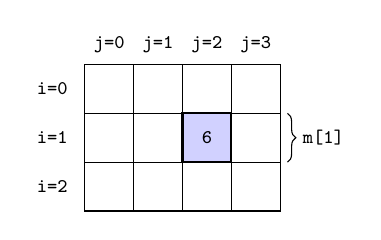
\begin{tikzpicture}[scale=0.62, every node/.style={font=\scriptsize\ttfamily}]
            % kolomnummers
            \foreach \j in {0,1,2,3}
            \node at (\j+0.5, 3.4) {j=\j};
            % rijnummers
            \foreach \i/\lab in {0/0, 1/1, 2/2}
            \node[anchor=east] at (-0.15, 2.5-\i) {i=\lab};
            % cellen
            \foreach \i in {0,1,2}
            \foreach \j in {0,1,2,3}
            \draw (\j, 2-\i) rectangle (\j+1, 3-\i);
            % gemarkeerde cel m[1][2]
            \fill[blue!18] (2, 1) rectangle (3, 2);
            \draw[thick] (2, 1) rectangle (3, 2);
            \node at (2.5, 1.5) {6};
            % rij 1 aanduiden
            \draw[decorate, decoration={brace, amplitude=3pt}, thin]
            (4.15, 2) -- (4.15, 1) node[midway, right, xshift=2pt] {m[1]};
        \end{tikzpicture}
    \end{center}
    \vspace{-2mm}
    \texttt{m[1][2] = 1 * 2 = 6}. \quad \texttt{m.length} is 3 (aantal rijen),
    \texttt{m[1].length} is 4 (aantal kolommen). Een rij zoals \texttt{m[1]} is zelf
    een gewone array.

    %--------------------------------------------------------
    \section{5. ArrayList}
    \begin{lstlisting}
private ArrayList<Ant> ants;
// in de constructor:
ants = new ArrayList<>();

ants.add(a);        // achteraan
ants.add(0, a);     // op index 0
ants.remove(i);     // op index
ants.remove(a);     // op object
ants.set(i, a);     // vervangen
ants.clear();       // alles weg

Ant b = ants.get(i);
int n = ants.size();
boolean k = ants.contains(a);
int j = ants.indexOf(a); // -1 als
boolean leeg = ants.isEmpty();

for (Ant a : ants)
{
    System.out.println(a);
}
\end{lstlisting}
    \texttt{size()} met haakjes, \texttt{length} zonder.

    %--------------------------------------------------------
    \section{6. Scanner}
    Het \texttt{try/catch}-blok krijg je op het examen. Wat je zelf moet weten is
    \textbf{wat er in de \texttt{while} komt}.

    \begin{center}
        \small
        \begin{tabular}{@{}ll@{}}
            \toprule
            \texttt{hasNext()}       & \texttt{next()}       \\
            \texttt{hasNextInt()}    & \texttt{nextInt()}    \\
            \texttt{hasNextDouble()} & \texttt{nextDouble()} \\
            \texttt{hasNextLine()}   & \texttt{nextLine()}   \\
            \bottomrule
        \end{tabular}
    \end{center}
    \texttt{next()} leest \'e\'en woord, \texttt{nextLine()} een hele regel. Er
    bestaat geen \texttt{nextChar()}: gebruik \texttt{next().charAt(0)}.

    \textbf{Bestand met afwisselend tekst en getal}, bv.\ \texttt{c Minoes 4}: lees
    in dezelfde volgorde als in het bestand.
    \begin{lstlisting}
while (sc.hasNext())
{
    String s = sc.next();
    char type = s.charAt(0);
    String naam = sc.next();
    int lft = sc.nextInt();
    dieren.add(maak(type, naam, lft));
}
// spatie en enter zijn hetzelfde:
// elke next... schuift een stukje op
\end{lstlisting}

    \textbf{Met puntkomma's} (\texttt{Minoes;4}):
    \begin{lstlisting}
String r = sc.nextLine();
String[] d = r.split(";");
int lft = Integer.parseInt(d[1]);
\end{lstlisting}

    %--------------------------------------------------------
    \section{7. Overerving}
    \begin{lstlisting}
public class Cat extends Animal
{
    private boolean tam;

    public Cat(String n, int lft,
               boolean tam)
    {
        // EERSTE regel, verplicht
        super(n, lft);
        this.tam = tam;
    }

    public boolean isTam()
    {
        return tam;
    }
}
\end{lstlisting}

    \textbf{Polymorfie.} In een \texttt{ArrayList<Animal>} mag ook een \texttt{Cat}
    zitten. Roep je \texttt{a.toString()} op, dan kiest Java \emph{zelf} de versie van
    het echte object. Je hebt dus geen \texttt{if (a instanceof Cat)} nodig.

    \begin{lstlisting}
// in de superklasse
public boolean juist(int i, char c)
{
    return antw[i] == c;
}

// in de subklasse
@Override
public boolean juist(int i, char c)
{
    if (joker.contains(i))
    {
        return true;
    }
    return super.juist(i, c);
}
\end{lstlisting}

    %--------------------------------------------------------
    \section{8. Zeven veelgebruikte methodes}

    \subsection{a. Zoeken $\rightarrow$ object of null}
    \begin{lstlisting}
public Ant zoek(String id)
{
    for (Ant a : ants)
    {
        if (a.getId().equals(id))
        {
            return a;
        }
    }
    return null;
}
\end{lstlisting}

    \subsection{b. Toevoegen $\rightarrow$ boolean}
    \begin{lstlisting}
public boolean voegToe(Ant nw)
{
    if (zoek(nw.getId()) != null)
    {
        return false;
    }
    ants.add(nw);
    return true;
}
\end{lstlisting}

    \subsection{c. Totaal / gemiddelde}
    \begin{lstlisting}
public double gemiddelde()
{
    // anders deling door 0
    if (ants.isEmpty())
    {
        return 0;
    }
    double som = 0;
    for (Ant a : ants)
    {
        som += a.getLoad();
    }
    return som / ants.size();
}
\end{lstlisting}

    \subsection{d. Grootste zoeken}
    \begin{lstlisting}
public Ant beste()
{
    Ant best = null;
    int max = -1;  // lager dan alles
    for (Ant a : ants)
    {
        if (a.getScore() > max)
        {
            max = a.getScore();
            best = a;
        }
    }
    return best;
}
\end{lstlisting}

    \subsection{e. Filteren $\rightarrow$ nieuwe lijst}
    \begin{lstlisting}
public ArrayList<Ant> vanJaar(int j)
{
    ArrayList<Ant> res =
        new ArrayList<>();
    for (Ant a : ants)
    {
        if (a.getJaar() == j)
        {
            res.add(a);
        }
    }
    return res;
}
\end{lstlisting}

    \subsection{f. Verwijderen $\rightarrow$ aantal}
    for-each $+$ \texttt{remove} $=$ crash. \texttt{it.next()} mag maar
    \'e\'en keer per ronde.
    \begin{lstlisting}
public int verwijder(int grens)
{
    int n = 0;
    Iterator<Ant> it =
        ants.iterator();
    while (it.hasNext())
    {
        Ant a = it.next();
        if (a.getScore() < grens)
        {
            it.remove();
            n++;
        }
    }
    return n;
}
\end{lstlisting}

    Of met een hulplijst:
    \begin{lstlisting}
public int verwijder(int grens)
{
    ArrayList<Ant> weg =
        new ArrayList<Ant>();
    for (Ant a : ants)
    {
        if (a.getScore() < grens)
        {
            weg.add(a);
        }
    }
    for (Ant a : weg)
    {
        ants.remove(a);
    }
    return weg.size();
}
\end{lstlisting}

    \subsection{g. Sorteren}
    \begin{lstlisting}
// selectiesortering, alfabetisch
for (int i = 0; i < l.size(); i++)
{
    int k = i;
    for (int j = i+1; j < l.size(); j++)
    {
        String x = l.get(j).getCode();
        String y = l.get(k).getCode();
        if (x.compareTo(y) < 0)
        {
            k = j;
        }
    }
    Item t = l.get(i);   // wisselen
    l.set(i, l.get(k));
    l.set(k, t);
}
// compareTo < 0 -> x komt eerst
// nooit met een for-each: je hebt
// de index nodig voor set(i, ...)
\end{lstlisting}

    Op twee dingen tegelijk (eerst \texttt{true}, dan alfabetisch): splits in twee
    lijsten, sorteer elk, en \texttt{addAll} ze na elkaar.

    %--------------------------------------------------------
    \section{9. Random}
    \begin{lstlisting}
import java.util.Random;

// veld, niet in een lus
private Random rn = new Random();

// 0 t.e.m. 9
int i = rn.nextInt(10);
// dobbelsteen 1 t.e.m. 6
int d = rn.nextInt(6) + 1;
// 0.0 tot 1.0
double x = rn.nextDouble();

// willekeurige letter uit tekst
String s = "abcd";
char c = s.charAt(
          rn.nextInt(s.length()));
\end{lstlisting}
    \texttt{nextInt(n)} stopt bij \texttt{n-1}. Voor \texttt{min} t.e.m.\
    \texttt{max}: \texttt{rn.nextInt(max-min+1) + min}.

    %--------------------------------------------------------
    \section{10. Objecten vergelijken}
    \texttt{==} werkt alleen als het letterlijk hetzelfde object is. Wil je weten of
    het dezelfde persoon is, vergelijk dan het veld dat uniek is.
    \begin{lstlisting}
// fout: vergelijkt adressen
if (k1 == k2) { }

// juist
if (k1.getNummer()
      .equals(k2.getNummer())) { }
\end{lstlisting}
    Let op de volgorde: \texttt{p.getNaam().equals("Bob")} crasht als \texttt{p}
    zelf \texttt{null} is. Check dan eerst \texttt{p != null \&\&}.

    %--------------------------------------------------------
    \section{11. UML (20\% van de punten)}
    \begin{center}
        \small
        \begin{tabular}{|l|}
            \hline
            \textbf{Kandidaat}                 \\ \hline
            $-$ mobielNummer : String          \\
            $-$ geboortejaar : int             \\ \hline
            $+$ Kandidaat(nr:String)           \\
            $+$ juist(i:int, c:char) : boolean \\ \hline
        \end{tabular}
    \end{center}
    \begin{itemize}
        \item Drie vakken: naam / attributen / methodes.
        \item $-$ = private, $+$ = public. Bij \emph{elk} lid.
        \item Altijd \texttt{naam : type}, en bij methodes alle parametertypes \'en het
              returntype. Daar staan de punten op.
        \item Constructor hoort bij de methodes.
        \item \texttt{static} = onderlijnd.
        \item Geerfde velden niet herhalen in de subklasse.
    \end{itemize}

    \textbf{De drie lijnen:}

    \begin{center}
        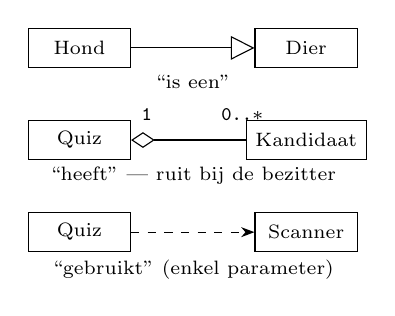
\begin{tikzpicture}[scale=0.9, font=\scriptsize,
                kl/.style={draw, minimum width=13mm, minimum height=5mm, font=\scriptsize}]

            % overerving
            \node[kl] (sub) at (0, 0) {Hond};
            \node[kl] (sup) at (3.2, 0) {Dier};
            \draw[-{Triangle[open, length=3mm, width=3mm]}] (sub) -- (sup);
            \node[anchor=north, font=\scriptsize] at (1.6, -0.25) {``is een''};

            % aggregatie
            \node[kl] (q) at (0, -1.3) {Quiz};
            \node[kl] (k) at (3.2, -1.3) {Kandidaat};
            \draw[{Diamond[open, length=3mm, width=2mm]}-] (q) -- (k);
            \node[anchor=south, font=\scriptsize\ttfamily] at (0.95, -1.16) {1};
            \node[anchor=south, font=\scriptsize\ttfamily] at (2.3, -1.16) {0..$\ast$};
            \node[anchor=north, font=\scriptsize] at (1.6, -1.55) {``heeft'' --- ruit bij de bezitter};

            % gebruikt
            \node[kl] (a) at (0, -2.6) {Quiz};
            \node[kl] (b) at (3.2, -2.6) {Scanner};
            \draw[dashed, -{Stealth}] (a) -- (b);
            \node[anchor=north, font=\scriptsize] at (1.6, -2.85) {``gebruikt'' (enkel parameter)};

        \end{tikzpicture}
    \end{center}

    \vspace{-2mm}
    De ruit staat bij de klasse die de lijst bezit.

\end{multicols}
\end{document}
